\documentclass{jsarticle}
\usepackage[dvipdfmx]{graphicx}
\title{電気化学測定法}

\author{03-190697 高松周平}
\date{\today}
\begin{document}
\maketitle
\section{実験の目的}
安定化ジルコニア固体電解質を用いた酸素濃淡電池の原理を理解するとともに、$\mathrm{Ni/NiO}$を標準極とする酸素濃淡電池の起電力を測定することにより、酸化鉄の標準生成Gibbsエネルギを求める。
\section{原理}
$$
E=\frac{RT}{4F}\ln{(\frac{p_{O_2}^R}{p_{O_2}^L})}
$$
$$
\Delta_{f}G_{Fe_xO}^{°}=\Delta_{f}G_{NiO}^{°}+2FE
$$
\section{手順}
\subsection{気体中の酸素分圧測定}
図1のような装置を用いる。そしてジルコニア管外側と内側の酸素の分圧に差をつけてあげればいいので、外側に酸素またはアルゴンガス、内側に空気を流し、600$〜$1000℃の範囲で起電力を測定する。\\
\begin{figure}[htbp]
 \begin{center}
  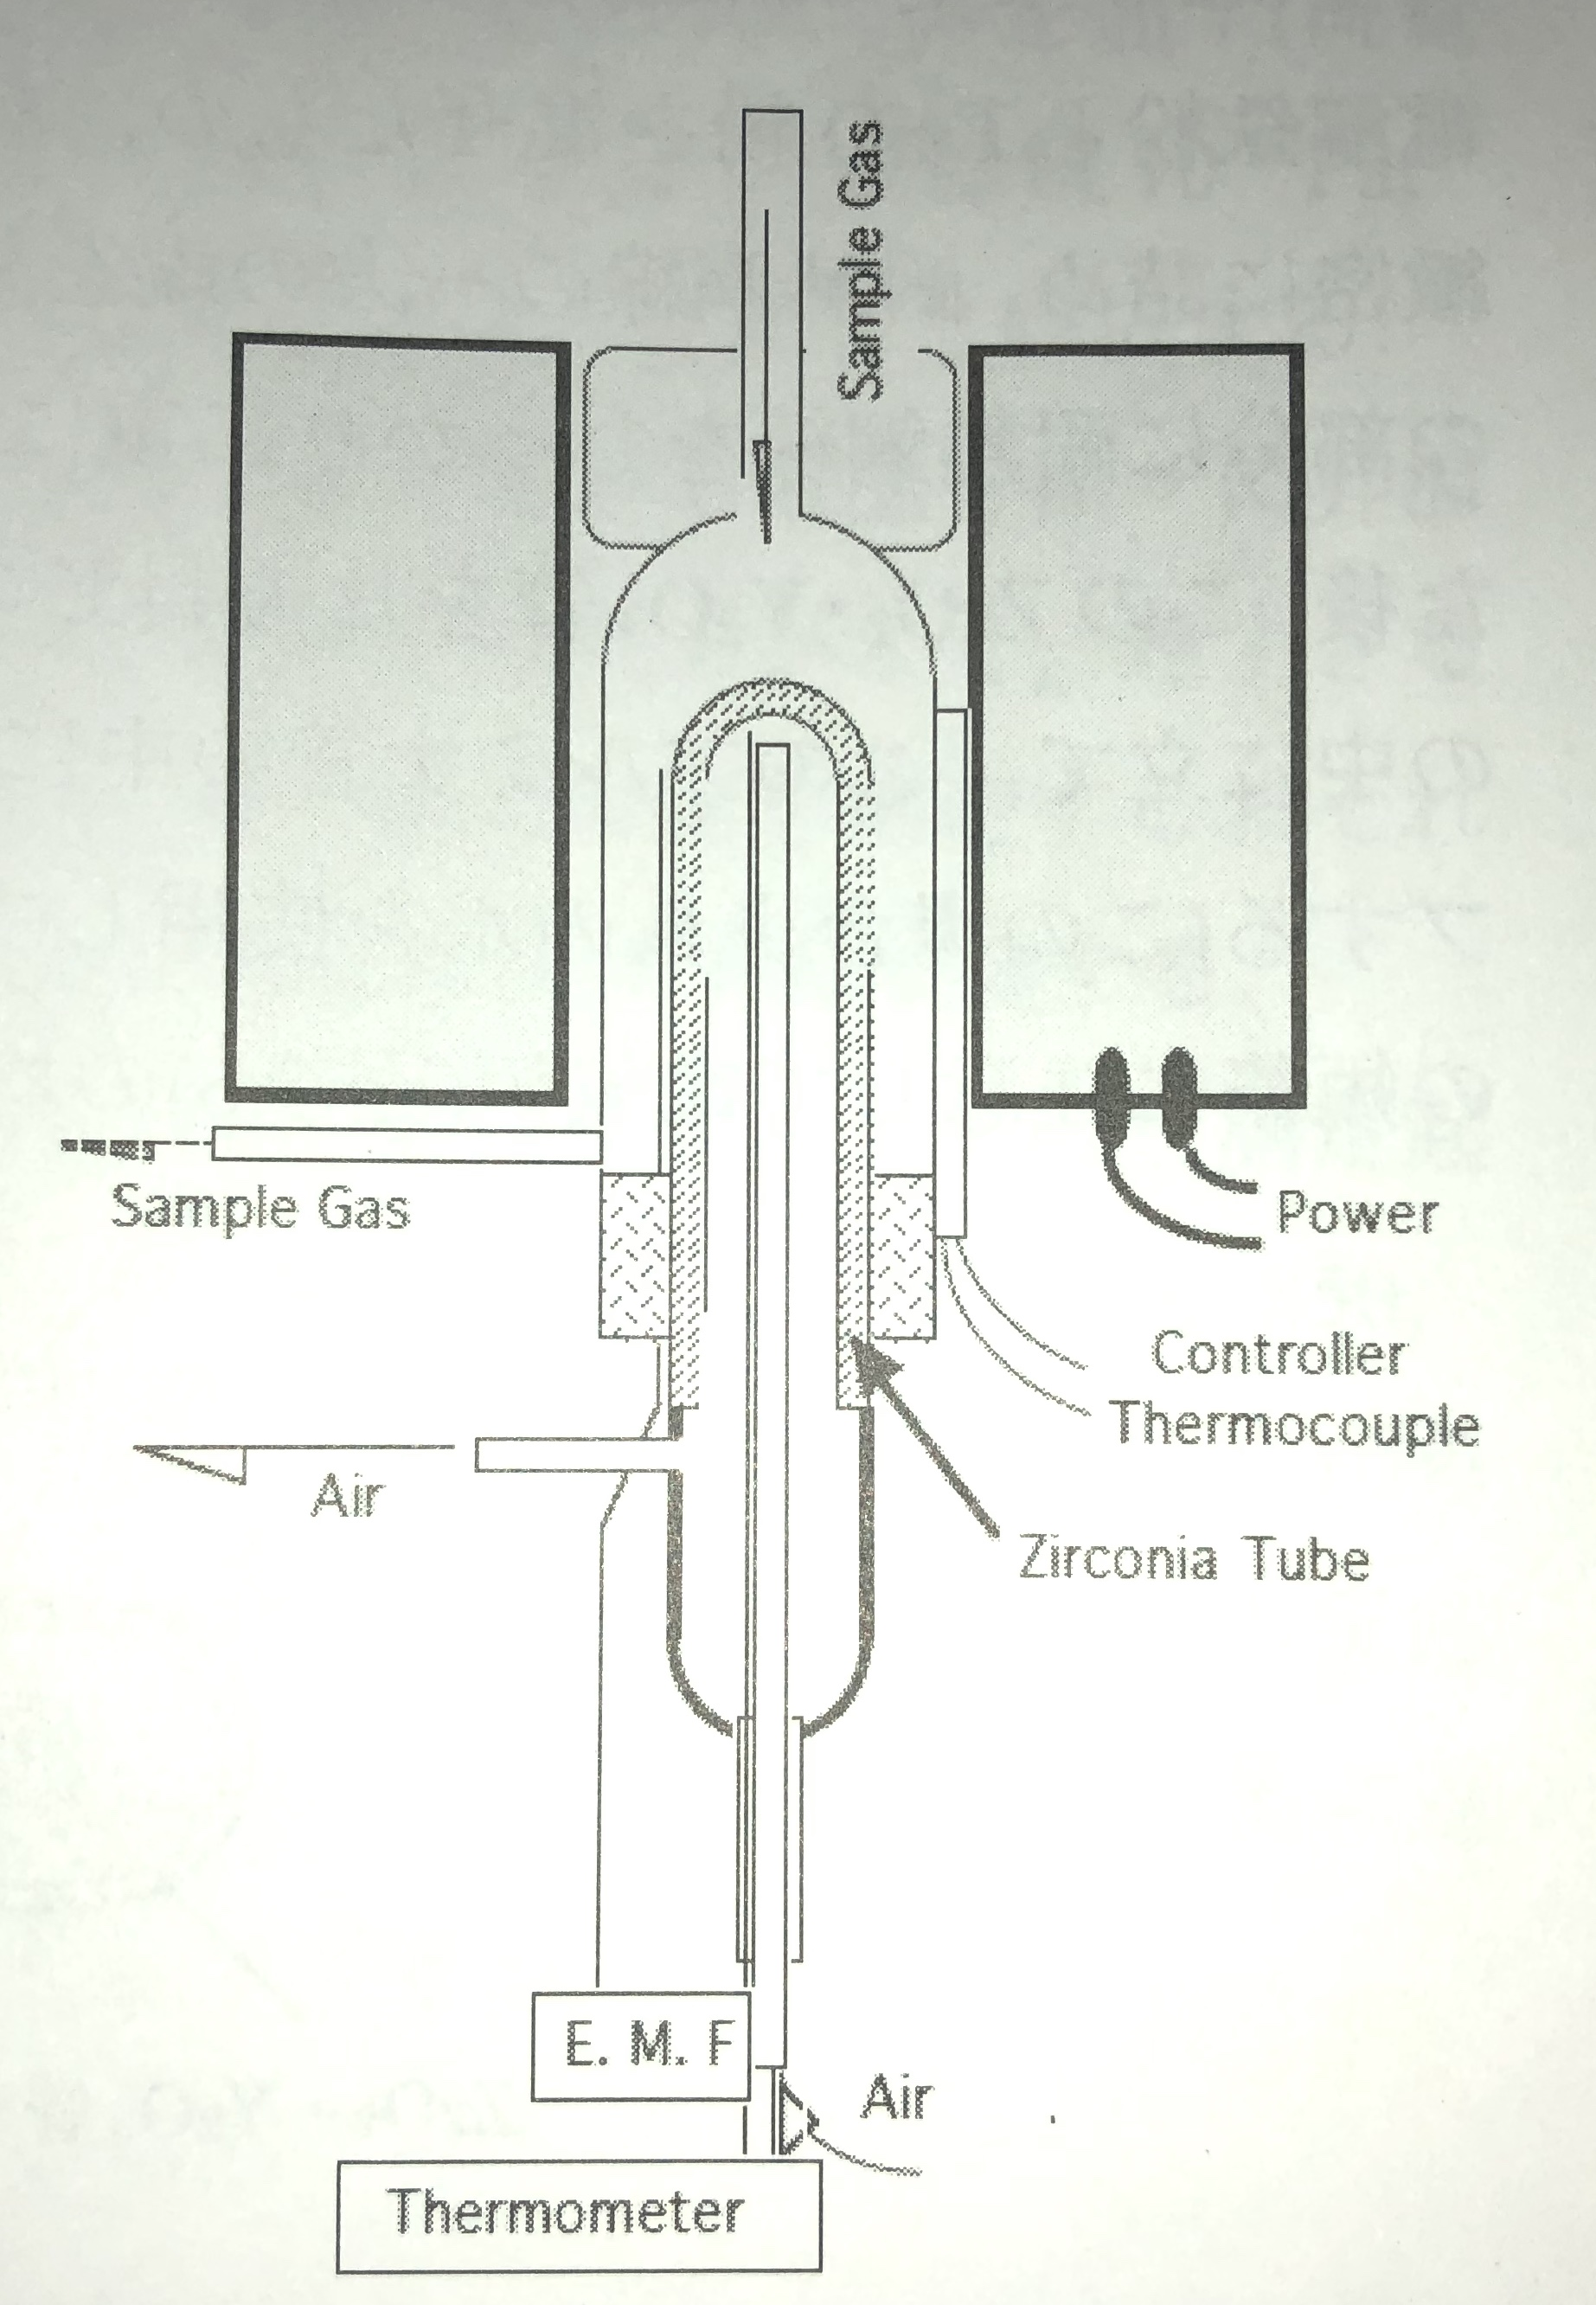
\includegraphics[width=50mm,height=70mm]{pictures/apparatus.png}
 \end{center}
 \caption{酸素濃淡電池型酸素センサの模式図}
 \label{fig:one}
\end{figure}
\subsection{$\mathrm{Fe_xOおよびFe_3O_4の標準生成Gibbsエネルギの測定}$}
片方封じの$\mathrm{ZrO_2}\cdot\mathrm{Y_2O_3}$管(外径8mm, 内径5mm, 長さ40mm)の内側に先端を和にした耐熱銅線(直径0.2mm)を底まで装入したものを2つ用意する。銅線の残りの一端は外に伸ばしておく。そして電解鉄粉と$\mathrm{Fe_xO}$粉を混ぜたもの、あるいは$Fe_xOとFe_3O_4$を混ぜたものをできるだけ緻密にそれぞれの管に詰める。次に管の外側の先端より約10mmの部分に耐熱銅線をしっかりと二重に巻きつけ内側の耐熱銅線と同じ方向に伸ばす。この管を片方封じのアルミナ管(外径20mm, 内径16mm, 長さ50mm)のなかの中央に立て、その周りに$\mathrm{Ni, NiO}$混合粉末(重量比1:1)をしっかりと押しつぶしながら詰め込む。最初に巻いた銅線が完全に混合粉末によって埋められるくらいまで詰め込んだら、こぼれないように上から綿を詰め込んで完成である。\\
\ \ \ このようにしてできたCellは空気中で昇温すると空気中の酸素によってNiと$\mathrm{Fe_xO及びFe_3O_4}$は用意に酸化されてしまうので電池全体をAr雰囲気において昇温する。750℃から初めて50℃刻みで900℃まで上げた後また750℃まで戻して測定する。所定の温度に達しても安定しているか確認するために5分待ち変化が$\pm0.5$mVならば安定していると判断する。
\section{結果}
\subsection{}
原理より
$$
E=\frac{RT}{4F}\ln{(\frac{p_{O_2}^R}{p_{O_2}^L})}=\frac{8.3144598\cdot T}{4\cdot96500}\ln{\frac{0.2}{1.0}}
$$
よって下の図のようになる。
\begin{figure}[htbp]
 \begin{center}
  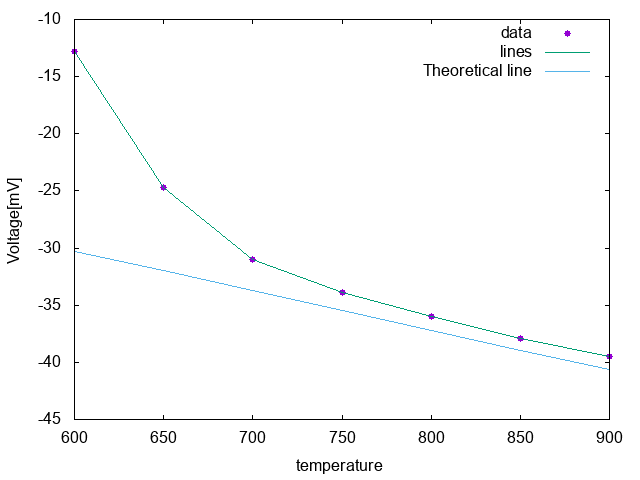
\includegraphics[width=70mm,height=50mm]{pictures/4-1.png}
 \end{center}
 \caption{測定した起電力及び理論起電力と温度の関係}
 \label{fig:one}
\end{figure}
\subsection{}
同様に原理より
$$
E=\frac{RT}{4F}\ln{(\frac{p_{O_2}^R}{p_{O_2}^L})}=\frac{8.3144598\cdot T}{4\cdot96500}\ln{\frac{0.2}{p_{O_2}^L}}
$$
で下図のようになる\\
\begin{figure}[htbp]
 \begin{center}
  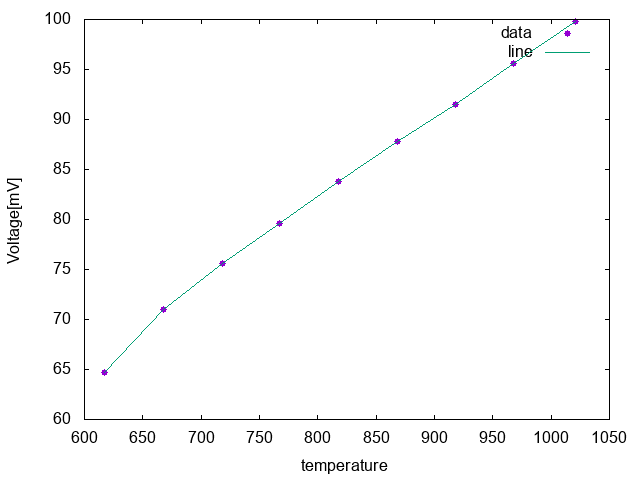
\includegraphics[width=70mm,height=50mm]{pictures/4-2.png}
 \end{center}
 \caption{測定した起電力と温度の関係}
 \label{fig:one}
\end{figure}
\\
これを最小二乗法でフィッティングすると傾きが$1.013\times10^{-1}$となるのでこれから逆算すると$ln{(\frac{0.2}{p_{O_2}^L})}=4702.87$となる。しかしこの値ではあまりに$\mathrm{p_{O_2}^L}$が小さいので計算できなかった、ほぼゼロとみなせる。\\
\subsection{}
原理より
$$
\Delta_{f}G_{Fe_xO}^{°}=\Delta_{f}G_{NiO}^{°}+2FE
$$
よって
\begin{table}[h]
\caption{}
 \label{table:SpeedOfLight}
 \centering
  \begin{tabular}{clll}
   \hline
   温度[℃] & $\Delta_{f}G_{Fe_xO}^{°}$ & $\Delta_{f}G_{Fe_3O_4}^{°} - (\frac{3}{x})\Delta_{f}G_{Fe_xO}^{°}$\\
   \hline \hline
   750 & -49614.2 & -89853.7\\
   800 & -50594.3 & -88955.0\\
   850 & -51593.7 & -87747.5\\
   900 & -52380.8 & -87003.2\\
   \hline
  \end{tabular}
\end{table}
\begin{figure}[htbp]
 \begin{center}
  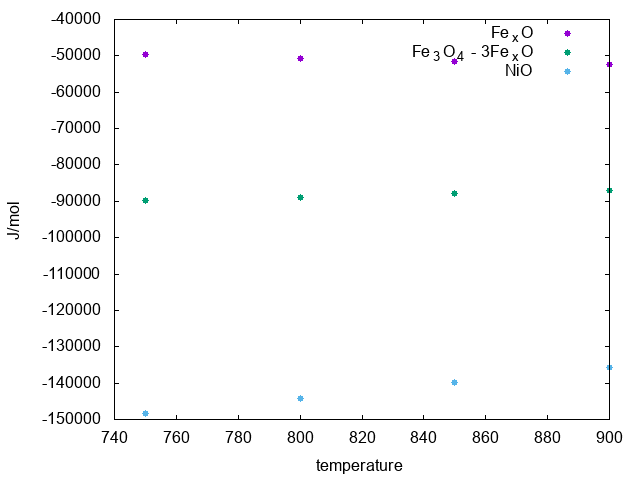
\includegraphics[width=70mm,height=50mm]{pictures/4-3.png}
 \end{center}
 \caption{}
 \label{fig:one}
\end{figure}
\\
\\
\begin{thebibliography}{99}
\bibitem{}  教科書
\end{thebibliography} 
\end{document}